\def\year{2018}\relax
%Taken from file: formatting-instruction.tex
\documentclass[letterpaper]{article} %DO NOT CHANGE THIS
\usepackage{aaai18}  %Required
\usepackage{times}  %Required
\usepackage{helvet}  %Required
\usepackage{courier}  %Required
\usepackage{url}  %Required
\usepackage{graphicx}  %Required
\frenchspacing  %Required
\setlength{\pdfpagewidth}{8.5in}  %Required
\setlength{\pdfpageheight}{11in}  %Required
%PDF Info Is Required:
%   \pdfinfo{
% /Title (Removing Viruses with Machine Learning in Dr.~Mario)
% /Author (Ryan Gately and JJ Brown)}

\usepackage{natbib}
\usepackage{url}
\usepackage{graphicx}

\author{Ryan Gately and JJ Brown}
\date{\today}
\title{Removing Viruses with Machine Learning in Dr.~Mario}

\bibliographystyle{aaai}

\renewcommand{\citet}[1]{\citeauthor{#1}~\shortcite{#1}}
\renewcommand{\citep}{\cite}
\renewcommand{\citealp}[1]{\citeauthor{#1}~\citeyear{#1}}

\begin{document}

\maketitle

\begin{abstract}
We trained machine learning agents that manipulate an NES controller to play Dr.~Mario by~\cite{drmario90}, using the FCEUX emulator by~\cite{fceux18}.
Both Q-learning and SARSA learning algorithms showed some advantage over a random controller.
We compared a SARSA agent that viewed the local ``neighborhood'' around the player's capsule and controlled the controller directly to a Q-learning agent that viewed the entire topmost layer of viruses and executed high-level actions in the game. Ultimately, while we believe the local ``neighborhood'' state space may allow for the highest theoretical quality of performance, the Q-learning agent with a high-level controller yielded the best results, with the fastest rate of learning and the highest average performance.
\end{abstract}

\section{Introduction}
Video games are an interesting application for developing machine learning agents beacuse the strictly-defined playing space provides a clean, simple environment for learning. Furthermore, they are also interesting such that they challenge the player to develop an effective strategy. We researchers, then, seek to determine whether a machine learning agent, using a simple learning algorithm, can effectively develop such strategies as to ``beat'' those games on par with a human, or if the game requires such skill as to mandate a human player.

We selected the classic video game ``Dr.~Mario'' by~\cite{drmario90} as the best candidate to develop a machine learning agent for, because we believed the simple yet challenging puzzle of dropping colored capsules would be viable for a machine learning agent to solve, yet difficult enough to force the agent to develop an effective strategy for winning.


\section{Problem Definition and Approaches}
\subsection{Task Definition}
We wanted to make machine learning agents that could play the classic video game ``Dr.~Mario'' for the Nintendo Entertainment System (NES). Therefore, we decided to use the FCEUX emulator, since it presented the most convenient interface between agent code and game actions. First, it has built in support for scripting with Lua​, which provides the agent with a way to execute actions and read the game state. Specifically, the game memory is polled periodically to retrieve values for the score, as well as location and type of blocks​ in the game area. Further, there is no hidden information that a human player would not see​: the agent only has access to information that would be displayed visually to a human. Finally, FCEUX provides a convenient way for Lua scripts to send commands to the emulator to emulate pressing a button on the NES controller. For these reasons, we decided to implement our agents in Lua scripts controlling the FCEUX emulator.

In Dr.~Mario, the player controls capsules with a color at each end that slowly fall down the screen, and tries to place the colored ends on ``virus'' blocks of the same color. If four blocks of the same color touch in a straight line, they are removed, and the player is awarded 200 points for any virus blocks removed in this way. Once the player removes all of the viruses on the screen, they complete the level and move to the next one. We wanted to train machine learning agents to complete at least one level, and outperform a ``random'' controller that presses a random button every frame.

\subsection{Algorithm Definition}
We developed two machine learning agents which learn using Q-learning and using SARSA. Each associates a value \(Q(s, a)\) with each possible state/action pair, and updates those values as it is rewarded or punished for taking an action \(a\) in a state \(s\).

For Q-learning, the value is updated after performing action \(a\) in state \(s\) to arrive in state \(s'\), yielding reward \(r\), with the following algorithm:
\begin{equation}
Q(s, a) \leftarrow Q(s, a) + \alpha * (r + \gamma * {\max}_{a'} Q(s', a') - Q(s, a))
\end{equation}

And similarly, SARSA updates values with the following algorithm:
\begin{equation}
Q(s, a) \leftarrow Q(s, a) + \alpha * (r + \gamma * Q(s', a') - Q(s, a))
\end{equation}
where the agent decides to perform action \(a'\) immediately upon arriving in state \(s'\), according to the current policy.

\section{Experimental Evaluation}
\subsection{Methodology}
We wanted to compare the effectiveness of an agent making high-level decisions versus one that manipulates the controller directly. We designed a Q-learning agent that would observe the colors of the highest block in each column as shown in Fig.~\ref{fig:high-level-state}, and use that to decide into which column (and with what orientation) the agent should drop the capsule. To carry out these high-level decisions, we made some simple algorithms to press buttons until the capsule was in the desired column and orientation, and then lower it into place. We believed that this high-level decision-making would be able to learn more quickly than a low-level approach, since it could achieve resutls in fewer steps. A single episode was concluded when the agent either won or lost a level.

\begin{figure}
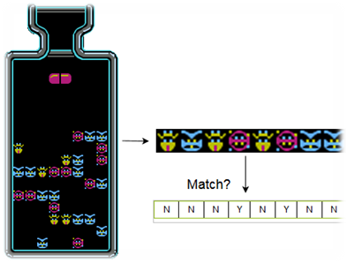
\includegraphics[width=0.5\textwidth]{high-level-state.png}
\caption{How the Q-learning agent extracts its state for high-level decision-making.}\label{fig:high-level-state}
\end{figure}

We also designed a SARSA agent that would observe only the blocks around it, and use that information to directly manipulate the controller. This agent perceived the highest blocks in the ``neighborhood'' of tiles within 2 tiles sideways and 5 below, and observed both the color and relative depth of those blocks as shown in Fig.~\ref{fig:local-state}. Using that information, the agent decided whether to move the player's capsule left, move it right, rotate it, or take no action. Similarly to the Q-learning experiment, an episode was concluded when the agent won or lost a level. Unlike that experiment, this agent made a decision once every frame, rather than once for each player capsule.

\begin{figure}
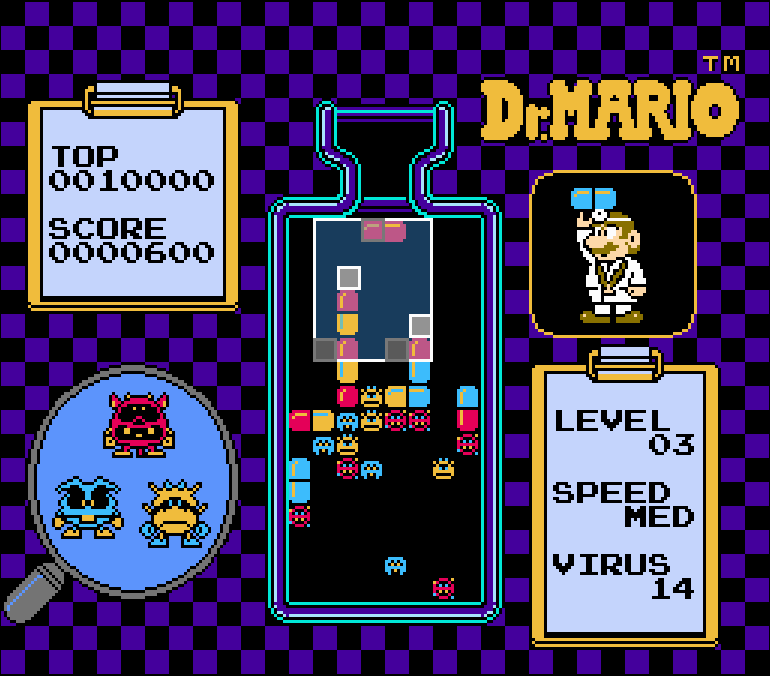
\includegraphics[width=0.5\textwidth]{local-state.png}
\caption{A representation of how the SARSA agent extracts its local state for low-level decision-making.}\label{fig:local-state}
\end{figure}

Both agents also performed some optimizations of state, in order to treat similar arrangements the same. For example, both agents observed not the exact color of each tile, but a presentation of four options: whether that tile matched the left part of the capsule, the right part, both, or neither. This way, a red capsule descending towards a red virus could be treated the same as a blue capsule descending towards a blue virus, and learning could be shared among similar states.

We also created a random controller, which would randomly decide each frame between pressing left, pressing right, rotating, or taking no action. We decided to compare the efficacy of each controller or agent by comparing the slope of how much more reward it earned per episode increased over time.

For each agent, we rewarded it 2000 points for removing a virus, punished it 50 points for losing a game, and punished it 1 point each time it made a decision to encourage the agent to try new actions over time. After each episode, we recorded the final game score, which is 2 time the number of viruses cleared.

The SARSA controller learned extremely slowly. We determined that part of the reason for this was that the default difficulty has very few viruses on the screen, and thus very little opportunity for an agent to accidentally clear a virus and earn points. Therefore, we learned from the SARSA experiment that we should start with a higher difficulty. The results from running the game at higher difficulty is presented below.

\subsection{Results}

We ran several experiments in each controller and compared the trend of how the game score increased with increasing episode number, as shown in Fig.~\ref{fig:random-results}. The random controller, predictably, did not improve over time; surprisingly, it did manage to clear one virus about once every four epsiodes on average.

\begin{figure}
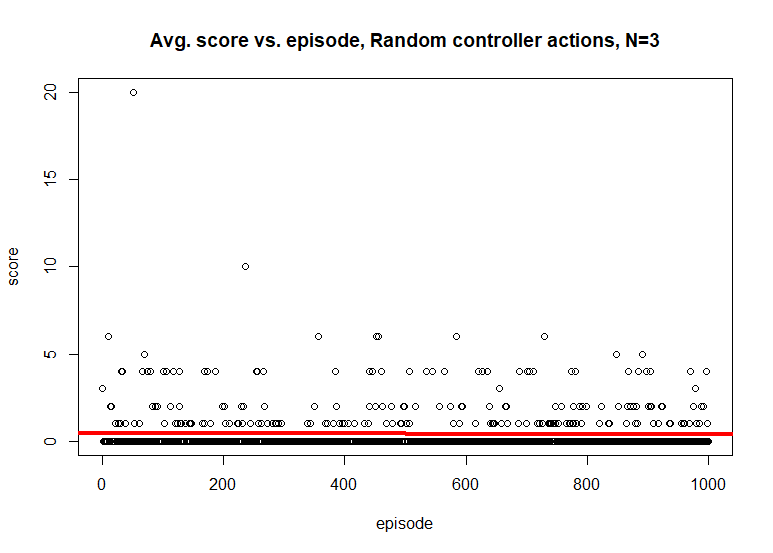
\includegraphics[width=0.5\textwidth]{random_results_n3.png}
\caption{Avg.~reward across 3 experiments for an episode vs.~episode number, with a random controller.}\label{fig:random-results}
\end{figure}

Despite starting at a higher difficulty, the SARSA agent with a local state learned very slowly, as shown in Fig.~\ref{fig:sarsa-results}. On average, it increased its score by 1.3e-5 points each episode. With this trend, it would only clear an additional virus off the screen every 7,500 attempts! As shown in Fig.~\ref{fig:sarsa-results}, the agent was often able to clear a single virus off the screen, but could not reliably remove more.

\begin{figure}
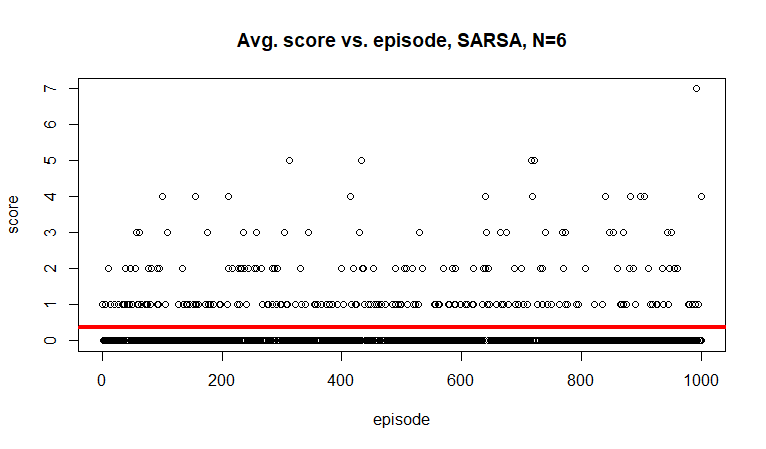
\includegraphics[width=0.5\textwidth]{sarsa_results_n6.png}
\caption{Avg.~reward across 6 experiments for an episode vs.~episode number, with a SARSA agent. While the slope appears to be zero, it is slightly positive (1.3e-5).}\label{fig:sarsa-results}
\end{figure}

The Q-learning agent learned much more quickly, often clearing 3 viruses at a time, but then plateued soon after it reached that level of skill. As shown in Fig.~\ref{fig:q-results}, the agent's typical behavior never improved beyond that point; however, it did actually manage to clear a level once, and its outlier behavior greatly outperformed both SARSA and the random controller.

\begin{figure}
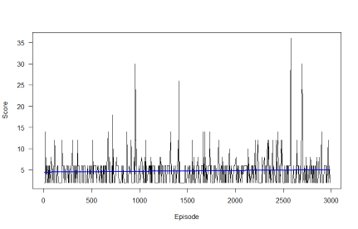
\includegraphics[width=0.5\textwidth]{q-learning-results.png}
\caption{Avg.~reward across for an episode vs.~episode number, with a Q-learning agent. Note the marked positive slope, and the spikes indicating occaisional very high performance.}\label{fig:q-results}
\end{figure}


\subsection{Discussion}
We found that a Q-learning agent making high-level decisions will outperform a SARSA agent making low-level decisions, at least for the first few thousand episodes. Both of those agents outperform an agent that presses buttons at random. Q-learning learns quickly, but doesn't improve much after that, while SARSA learning shows slow, steady improvement over time. As we discuss in Section~\ref{sec:future-work}, if we can encourage the agents with more frequent rewards, we expect both of them to make further and quicker progress.

\section{Related Work}

\section{Future Work}\label{sec:future-work}
In the future, we think we could improve the efficacy of the learning algorithms by rewarding agents for accomplishing sub-goals as discussed in~\cite{banzas15} and~\cite{bhonker17}, such as rewarding the agent for matching smaller numbers of matching colors or for matching a series of only capsule blocks (which the game does not reward), rather than only rewarding it for making matches that include colored virus blocks.

\section{Conclusion}

\newpage

\bibliography{report}

\end{document}